\documentclass[letterpaper]{book}
%permite agregar codigo fuente
\usepackage{listings}
\lstset{language=c++,
		showstringspaces=false,
		 breaklines=true}
\usepackage{graphicx}
%establece los limites de la numeracion de capitulos
\setcounter{secnumdepth}{4}
\setcounter{tocdepth}{4}
\title{UDG\_PololuMaestro User guide}
\author{Omar Alejandro Rodr\'{i}guez Rosas}

\begin{document}


\maketitle

\tableofcontents
\chapter{Introduction}
This library provides a hardware abstraction class to easily control the Pololu Maestro board. The current implementation supports servo outputs only, other features of the board sucha as general purpose PWM or digital/analog I/O are not yet available.\\
This guide assumes some degree of familiarity with the board itself an its features. It is strongly suggested that you read the Pololu Maestro's user guide before continuing any further with this document.\\

\chapter{Setup}
\section{Preparing your environment}
1. Follow the instructions on the user guide to install Maestro Control Center, available for Linux and Windows. If using windows you might need to install a driver for the board.\\
2. Connect the board to your computer. If you're using ubuntu it is possible that an error flag on the Maestro activates (you'll see a red LED turn on). This behavior is expected and you can turn it off at the error tab on Maestro Control Center.\\
3. Open Maestro Control Center an make sure that the cannels you intend to use are enabled on the Status tab (see figure \ref{fig:maestro1}).\\
\begin{figure}
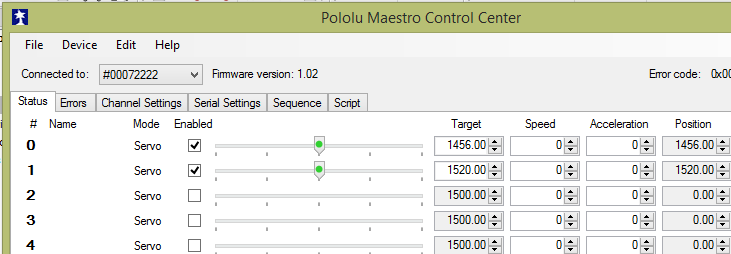
\includegraphics[width=\textwidth]{images/maestro1.png}
\caption{Status tab of the Maestro Control Center}
\label{fig:maestro1}

\end{figure}
4. For safety reasons, it is important to verify that the min and max pulse widths allowed by the board match with those actually supported by your servos. These limits are usually provided by the vendor. You can verify this on the Channel settings tab at the Maestro Control Center (see figure \ref{fig:maestro2}).\\
5. Connect the servos to the channel of your choice (see the Maestro's user guide for the layout of your specific board). Remember the channel numbers since they need to be explicitly declared in the code. Don forget to plug the DC supply for your servos (see the Maestro's user guide).\\
\begin{figure}
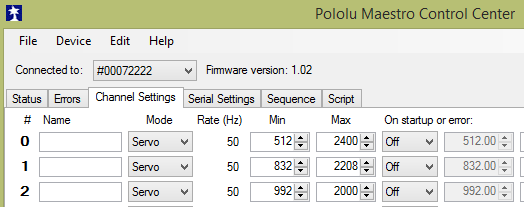
\includegraphics{images/maestro2.png}
\caption{Channel settings tab of the Maestro Control
\label{fig:maestro2}
 Center}
\end{figure}


\section{Building with UDG\_PololuMaestro}
This guide uses Microsoft Visual Studio Express for Desktop 2012 and Windows 8.1 or g++ 4.7 and Ubuntu 13.10. Other compiler/OS/Distribution combnations might work as well but haven't been tested.\\
\subsection{Windows}
1. Copy the UDG\_PololuMaestro release folder to a suitable location.\\
2. Open your Visual Studio solution.\\
3. As an optional step, you might want to add UDG\_PololuMaestro include (\textless{}Release\_Folder \textgreater\textbackslash{include}) and library (\textless{}Release\_Folder\textgreater\textbackslash{include}\textbackslash{bin}\textbackslash{\textless{}Architecture\textgreater}) directories to your default search folders. To do so, for the include folder go to Project\textbackslash{\textless{}Name\textgreater Properties}\textbackslash{Configuration Properties}\textbackslash{C/C++}\textbackslash{General} and enter the appropriate path in Additional Include Directories. Similarly, for the binary folder edit the Additional library directories property in  Project\textbackslash{\textless{}Name\textgreater{}Properties}\textbackslash{Configuration Properties}\textbackslash{Linker}\textbackslash{General}.\\
4. Your source files should use \#include \textless UDG\_PololuMaestro.h\textgreater or \#include ``UDG\_PololuMaestro.h''\footnote{Remember that, when using quotes, If the header file is not on your current directory the full path should be included i.e. \#include ``c:\textbackslash{}foo\textbackslash{}bar\textbackslash{}UDG\_PololuMaestro.h''.}\\
5. Make sure you're linking with UDG\_PololuMaestro.lib. To do so add UDG\_PololuMaestro.lib to Additional Dependencies in Project\textbackslash{\textless{}Name\textgreater{}Properties}\textbackslash{Configuration Properties}\textbackslash{Linker}\textbackslash{Input} or add \#pragma comment(lib,``UDG\_PololuMaestro.lib'') to your code. \footnote{Use the whole path if you skipped step 3.}\\
6. In order for UDG\_PololuMaestro to work, serial settings of the board must be USB Dual Port. You can verify this at the serial settings tab on Maestro Control Center.\\
\subsection{Linux (Ubuntu)}
1. Copy the UDG\_PololuMaestro release folder to a suitable location.\\
2. As an optional step you might want to place the header and library files into your default search directories. Typically you'll need to copy \textless{}Release\_Folder\textgreater{}/include/UDG\_PololuMaestro.h to /usr/include/ and \textless{}Release\_Folder\textgreater{}/bin/\textless{}Architecture\textgreater{}/libUDG\_PololuMaestro.a to /usr/lib.\footnote{These default libraries might vary depending on your compiler settings.}\\
3. Your source files should use \#include \textless UDG\_PololuMaestro.h\textgreater or \#include ``UDG\_PololuMaestro.h''\footnote{Remember that, when using quotes, If the header file is not on your current directory the full path should be included or you can also use the -I option (see g++ help).}\\
4. To build your application use -std=c++11 \footnote{ -std=c++0x might work as well if you're using an older g++ version} and link with -lUDG\_PololuMaestro.a \footnote{Or simply UDG\_PololuMaestro.a if you skipped step 2. If the file is not on your current folder you can use its whole path or the -L option (see g++ help).}


\chapter{The UDG\_PololuMaestro API}
\section{PololuMaestro class}
Provides a software abstraction for the PololuMaestro board

\subsection{public members}

\subsubsection{PololuMaestro(HANDLE fd)}
\label{sec:constructor1}
This constructor method initializes the PololuMaestro using the provided Serial Port descriptor. By default, the number of channels is set to 18 (assumes Pololu Maestro 18 board). For a different number of channels, use PololuMaestro(HANDLE, int).
\textbf{HANDLE fd:} A file descriptor for a Serial Port (COM ports in windows, /dev/tty in linux). You can get a file descriptor using the following function:\\\\
\textbf{Windows}
\begin{lstlisting}
HANDLE OpenSerialPort(LPWSTR name)
{
	HANDLE portDescriptor;
	DCB deviceControlBlock;
	portDescriptor = CreateFile(name,
				GENERIC_READ|GENERIC_WRITE,
				0,0,OPEN_EXISTING,0,0);
	if(portDescriptor == INVALID_HANDLE_VALUE)
	{
		printf("Failed opening %ls\n", name);
		return INVALID_HANDLE_VALUE;
	}

	FillMemory(&deviceControlBlock,sizeof(DCB),0);
	deviceControlBlock.DCBlength = sizeof(DCB);
	if(BuildCommDCB(L"57600,n,8,1",&deviceControlBlock))
	{
		printf("Successfully configured DCB!\n");
		
	}
	else
	{
		printf("Something went wrong while building the DCB\n");
		return INVALID_HANDLE_VALUE;
	}

	if (!SetCommState(portDescriptor,&deviceControlBlock))
	{
		printf("Error configuring port\n");
		return INVALID_HANDLE_VALUE;
	}
	else
	{
		printf("Serial port ready\n");
	}
		
	return portDescriptor;
}
\end{lstlisting}
\textbf{\\\\Linux}
\begin{lstlisting}
int OpenSerialPort(const char* device)
{
	int fd = open(device, O_RDWR | O_NOCTTY);
	struct termios options;
	tcgetattr(fd, &options);
	options.c_lflag &= ~(ECHO | ECHONL | ICANON | ISIG | IEXTEN);
	options.c_oflag &= ~(ONLCR | OCRNL);
	tcsetattr(fd, TCSANOW, &options);
	return fd;
}
\end{lstlisting}
\subsubsection{PololuMaestro(HANDLE fd,int nchannels)}
This constructor method initializes the PololuMaestro using the provided Serial Port descriptor.The number of channels is set to \textit{nchannels}. You should set \textit{nchannels} accordingly to your board (18 for Maestro 18, 24 for Maestro 24, etc.).\\
\textbf{HANDLE fd:} A file descriptor for a Serial Port (COM ports in windows, /dev/tty in linux (See \ref{sec:constructor1} for a code sample).\\
\textbf{int nchannels:} The number of channels on your board.\\

\subsubsection{~PololuMaestro()}
Destructor method of the class. Cleans all of the resources requested by the class.\\

\subsubsection{	bool SetAngle(int channel, float angle)}
Approximates the position specified by \textit{angle} for the motor connected to \textit{channel} based on the constraints specified by the ServoMotor class instance at channels[\textit{channel}] (see \ref{sec:ServoMotor} ). The appropriate pulse to achieve \textit{angle} is calculated using $\frac{a+r}{2r}(p_{max} - p_{min}) + p_{min}$ where $a$ is the angle specified by \textit{angle}, $r$ is the movement range of the servo, $p_{max}$ is the max pulse supported by the servo and $p_{min}$ is the servo's minimum pulse. If $\left|angle\right|$ is greater than $\left|r\right|$, $a$ is capped to $\pm r$.\\
\textbf{int channel: }The channel where the desired motor is connected.\\
\textbf{float angle: } Signed angle in degrees relative to the neutral position.\\\\
\textbf{Return value: }true if the operation suceeds, false if it doesn't.\\

\subsubsection{float GetAngle(int channel)}
Gets the approximate position in degrees of the motor connected at \textit{channel}, relative to its neutral position. This angle is approximated using $\frac{p - p_{min}}{p_{max}-p_{min}}2r - r$  where $p$ is the current pulse at \textit{channel}, $r$ is the movement range of the servo, $p_{max}$ is the max pulse supported by the servo and $p_{min}$ is the servo's minimum pulse.\\\\
\textbf{Return value:} The approximate motor position in degrees relative to the neutral position.

\subsubsection{bool SetTarget(int channel,unsigned short targetUs)}
Sets \textit{targetUs} as the pulse at channel \textit{channe}. If \textit{targetUS} is outside the range of the motor range (specified at the associated ServoMotor class instnace) the value is capped to the appropriate max or min value.\\
\textbf{int channel: }the number of the channel to set.\\
\textbf{unsigned short targetUs: } target pulse in $\mu$s.\\\\
\textbf{Return value: } true if the operation succeeds, false if it doesn't.

\subsubsection{bool SetSpeed(int channel,unsigned short speed)}
Limits the speed at which a servo connected to \textit{channel} changes its output value. The speed limit is given in units of
(0.25 $\mu$s)/(10 ms) by \textit{speed}. A speed of 0 makes the speed unlimited, so that setting the target will immediately affect the position.
Note that the actual speed at which your servo moves is also limited by the design of the servo itself, the supply
voltage, and mechanical loads; this parameter will not help your servo go faster than what it is physically capable of.
At the minimum speed setting of 1, the servo output takes 40 seconds to move from 1 to 2 ms.\\

\textbf{int channel: }the number of the channel to set.\\
\textbf{unsigned short speed: } the speed limit in units of
(0.25 $\mu$s)/(10 ms)\\\\
\textbf{Return value: } true if the operation succeeds, false if it doesn't.

\subsubsection{bool SetAcceleration(int channel,unsigned short acceleration)}
Limits the acceleration of the servo connected to \textit{channel}. The acceleration limit is a value from 0 to 255
in units of (0.25 $\mu$s)/(10 ms)/(80 ms) specified by \textit{acceleration}. A value of 0 corresponds to no acceleration limit. An acceleration limit causes the speed of a servo to slowly ramp up until it reaches the maximum
speed, then to ramp down again as position approaches target, resulting in a relatively smooth motion from one point
to another.\\
\textbf{int channel: }the number of the channel to set.\\
\textbf{unsigned short acceleration: } the acceleration limit in units of
(0.25 $\mu$s)/(10 ms)\\\\
\textbf{Return value: } true if the operation succeeds, false if it doesn't.

\subsubsection{unsigned short GetPosition(int channel)}
Gets to current pulse at \textit{channel}.\\
\textbf{int channel: } the channelto get the pulse with from.\\\\
\textbf{Return value: } The current pulse width of the selected channel.

\subsubsection{bool AssignChannel(int channel, ServoMotor motor)}
Assigns the ServoMotor instance \textit{motor} to channel \textit{channel}. The information provided by this instance will be used to determine important security and operational constraints.

\textbf{int channel: }the number of the channel to be assigned.\\
\textbf{ServoMotor motor: } An abstraction of the motor being used\\\\
\textbf{Return value: } true if the operation succeeds, false if it doesn't.

\subsubsection{bool IsMoving()}
Indicates if there is at least one channel that hasn't reached its target position. This command works properly only with speed or acceleration constrained channels. \\\\
\textbf{Return value: } true if there is at least one channel that hasn't reached it target pulse, false if  it doesn't.

\subsection{Private members}

\subsubsection{HANDLE deviceDescriptor}
A file descriptor associated to the device serial communication port. HANDLE type is defined as int in linux.
\subsection{	ServoMotor* channels}
An abstraction of the Maestro's channels. Memory for this array is allocated at runtime and it's freed in the destructor method.

\subsubsection{int numberOfChannels}
The number of channels on the board. Thi is set at the constructor method and must match the number of physically available channels on the board.

\subsubsection{bool WriteToDevice(unsigned char* buffer, int nBytes)}
Writes \textit{nBytes} bytes from \textit{buffer} to the associated \textit{deviceDescriptor}. Returns true if the operation succeeds, false if it doesn't.

\subsubsection{bool ReadFromDevice(unsigned char* buffer, int nBytes)}
Reads \textit{nBytes} bytes from the associated \textit{deviceDescriptor} into \textit{buffer}. Returns true if the operation succeeds, false if it doesn't.

	

\section{ServoMotor class}
\label{sec:ServoMotor}
\subsection{int minPulse}
The servo's minimum pulse width in $\mu$s.
\subsection{int maxPulse}
The servo's max supported pulse width in $\mu$s.
\subsection{int neutralPulse}
The servo's max supported pulse width in $\mu$s.
\subsection{int degreeRange}
The amount of degrees the servo can move from it neutral position its max or minimum (i.e. for 180° servo degreeRange = 90).

\subsection{int AngleToPulse(float angle)}
Converts \textit{angle} to its equivalent pulse width according to the class parameters.\\
\textbf{float angle: }The (signed) angle to convert.\\\\
\textbf{Return value: }The equivalent pulse width for \textit{angle}.
\subsection{void SetParameters(int \_minPulse, int \_maxPulse, int \_neutralPulse, int \_degreeRange)}
Sets values for the servo's parameters.\\
\textbf{int \_minPulse} The value of minPulse.\\
\textbf{int \_maxPulse} The value of maxPulse.\\
\textbf{int \_neutralPulse} The value of neutralPulse.\\
\textbf{int \_degreeRange} The value of degreeRange.

\chapter{Code Samples}
The code samples work for the Microsoft c++ compiler (cl, using Visual Studio Express 2012 for desktop) and g++ 3.8. Other compilers might work as well but haven't been tested yet. Windows examples assume an unicode build. \\
\section{Opening a serial port descriptor}
For both Linux and Windows implementations, you need to provide a file descriptor associated with a serial port. The following samples demonstrate how to code a function to do so.\\
textbf{NOTE: }The name of the serial port associated with your board varies from system to system. You'll notice that two virtual communication ports with contiguous numbering will register themselves when connecting the board. You need to use the one with the higher number. Typically this will be COMx for Windows and ttyACMx for linux.\\
\subsection{Windows}
\begin{lstlisting}

HANDLE OpenSerialPort(LPWSTR name)
{
	HANDLE portDescriptor;
	DCB deviceControlBlock;
	portDescriptor = CreateFile(name,
				GENERIC_READ|GENERIC_WRITE,
				0,0,OPEN_EXISTING,0,0);
	if(portDescriptor == INVALID_HANDLE_VALUE)
	{
		printf("Failed opening %ls\n", name);
		return INVALID_HANDLE_VALUE;
	}

	FillMemory(&deviceControlBlock,sizeof(DCB),0);
	deviceControlBlock.DCBlength = sizeof(DCB);
	if(BuildCommDCB(L"57600,n,8,1",&deviceControlBlock))
	{
		printf("Successfully configured DCB!\n");
		
	}
	else
	{
		printf("Something went wrong while building the DCB\n");
		return INVALID_HANDLE_VALUE;
	}

	if (!SetCommState(portDescriptor,&deviceControlBlock))
	{
		printf("Error configuring port\n");
		return INVALID_HANDLE_VALUE;
	}
	else
	{
		printf("Serial port ready\n");
	}
		
	return portDescriptor;
}

\end{lstlisting}
\subsection{Linux}
\textbf{NOTE: }In the linux implementation, HANDLE is defined as int.\\
\begin{lstlisting}
int OpenSerialPort(const char* device)
{
	int fd = open(device, O_RDWR | O_NOCTTY);
	struct termios options;
  tcgetattr(fd, &options);
  options.c_lflag &= ~(ECHO | ECHONL | ICANON | ISIG | IEXTEN);
  options.c_oflag &= ~(ONLCR | OCRNL);
  tcsetattr(fd, TCSANOW, &options);
  return fd;
}
\end{lstlisting}
\section{Typical applications}
This section presents typical use cases and some basic operations.
\subsection{Initialize Servo and PololuMaestro objects}
Once a serial port is open, you need to initialize a ServoMotor object (matching the features of your physical servo). Then you'll assign that servo to a maestro channel.\\
\begin{lstlisting}
#include "UDG_PololuMaestro.h"
//OpenSerialPort() definition
//{...}
int main()
{
fd = OpenSerialPort(PortName);
ServoMotor motor;
motor.SetParameters(992,//min pulse
		   2000,//max pulse
		   1500,//neutral pulse
		   90//degree range
		   );
PololuMaestro maestro(fd,
		   18//number of channels on the board
		   );
maestro.AssignChannel(0,motor); //assign to channel 0
return 0;
}
\end{lstlisting}
\subsection{Moving the servos: blocking and non-blocking}
To change the position of your servos, you can use PololuMaestro::SetTarget() and PololuMaestro::SetAngle(). Remember that both functions will return immediatly even if the position hasn't been physically reached. To avoid this you can set a speed or acceleration limit (or both) and use PololuMaestro::isMoving() function to wait until all motors reach their position. This sample demonstrates both possibilities.\\
\begin{lstlisting}
#include "UDG_PololuMaestro.h"
//OpenSerialPort() definition
//{...}
int main()
{
fd = OpenSerialPort(PortName);
ServoMotor motor;
motor.SetParameters(992,2000,1500,90);
PololuMaestro maestro(fd,18);
maestro.AssignChannel(0,motor);
//Go to neutral position
maestro.SetTarget(0,motor.neutralPulse);
//function returns immediately, you might want
//to include a Sleep/Delay routine

//set a speed limit of 20
maestro.SetSpeed(0,20);
//Set an angle as target and wait until is reached
float angle = 45;
maestro.SetAngle(0,angle);
while (maestro.IsMoving());

return 0;
}
\end{lstlisting} 

\end{document}